\section{Delay}
Delay is an audio effect which memorize the input signal for a customized time, and then release the signal without change the signal. The delayed signal can ether be played back multiple times witch make echo, or only delay the signal for the specified time. When the signal is delayed and played back multiple times, the delayed signal must be attenuated, unless the signal will keep moving in infinity time and depending on component tolerance, the delayed signal will be amplified or attenuated. If the delay is amplified the signal will start oscillate, so in analog delay unit the delayed signal needs to be attenuated to avoid oscillation. The \autoref{fig:delay_block} shows a block diagram over a simple delay, "echo" unit.


\begin{figure} [htbp]
 \centering
  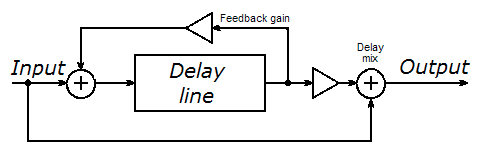
\includegraphics[width=0.8\textwidth]{delay_block}
  \caption{The photo shows a block diagram on a delay unit}
  \label{fig:delay_block}
\end{figure}

The \autoref{fig:delay_block} shows a delay unit with feedback line, where the gain is adjusted. The feedback signal is attenuated and added to the delay line. This will continue until the signal is completely attenuated. This kind of delay give the echo effect, and this effect is the delay effect in guitar effect unit. The following \autoref{fig:delay_echo} shows the effect in time domain.

\begin{figure} [htbp]
 \centering
  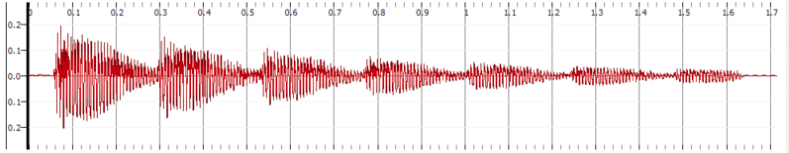
\includegraphics[width=1\textwidth]{delay_echo}
  \caption{The photo shows a echo in time domain}
  \label{fig:delay_block}
\end{figure}

http://www.hobby-hour.com/guitar/delay_effects.php